\chapter{Aufgabe 9}
\section{Algorithmus zur Bestimmung der Samplingrate}
Um die Samplingrate der Aufnahme des Oszilloskops zu bestimmen, sollte zunächst die Periodendauer T berechnet werden.
Da die Frequenz f hier bekannt ist geht dies über die Beziehung T = $\frac{1}{T}$ .
Nun muss die Anzahl N der Samples pro Periode festgestellt werden.
Dazu muss die Anzahl der Messwerte zwischen zwei Minima bestimmt werden.
Anschließend kann die Samplingrate SR mit der Beziehung SR = $\frac{N}{T}$ berechnet werden.
Fasst man beide Formeln zusammen führt dies zu der Beziehung SR = N $\cdot$ f .
Der Algorithmus ist als Ablaufdiagramm in Abbildung \ref{algo1} zusehen. \par 

\begin{figure}[h]
	\centering
	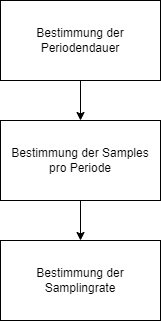
\includegraphics[scale=0.5]{Images/aufgabe9_algo1.png}
	\caption{Ablaufdiagramm des ersten Algorithmus der Aufgabe 9}
	\label{algo1}
\end{figure}

\subsection{Aktualisierung}
Nach dem Versuch das über diesen simplen Ansatz zu Implementieren haben sich einige Probleme aufgetan.
Die aufgenommenen Daten des Oszilloskop sind sehr genau und müssen genauer ausgewertet werden um ein Minima festzustellen.
Deswegen wurden einige Überlegungen zur Anpassung des Algorithmus vorgenommen.\par
Zunächst wurde das einlesen der Daten angepasst.
Die Daten sollten in einem zweidimensionalem Array eingelesen werden, damit Samplingnummern und Werte zueinander zugeordnet werden können.
Die Daten werden eingelesen und in diesem Array gespeichert.\par
Um die Minimas zu bestimmen wird nun der erste niedrigste Wert bestimmt.
Anschließend muss, um das zweite Minima zu bestimmen, abgewartet werden bis die Werte wieder ansteigen, um sicher zu stellen das das zweite Minima auch einer kompletten Periode entspricht.
Dafür wurde ein Schwellenwert von Zwei festgelegt, da die Schwankungen sich nur um eins unterscheiden.\par
Mithilfe der Werte im Array kann nun die Anzahl der Samples zwischen diesen beiden Punkten festgestellt werden.
Die Auswertung und Berechnung der Samplingrate erfolgt wie zuvor beschrieben.\par
Der angepasste Algorithmus ist in Abbildung \ref{algo1.1} zu sehen.

\begin{figure}[h]
	\centering
	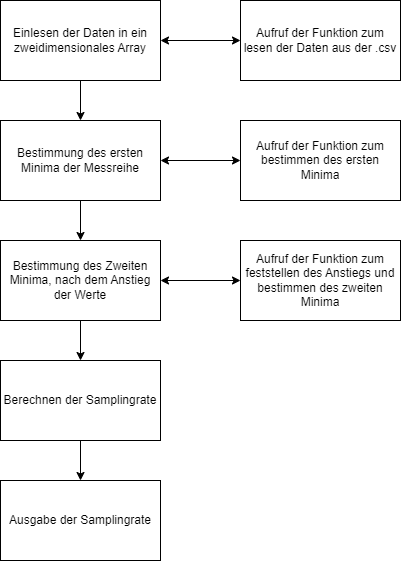
\includegraphics[scale=0.5]{Images/aufgabe9_algo1.1.png}
	\caption{Aktualisiertes Ablaufdiagramm des ersten Algorithmus der Aufgabe 9}
	\label{algo1.1}
\end{figure}

\section{Algorithmus zur Bestimmung der Frequenz}
Da in der Aufgabe keine Samplingrate angegeben ist, nehme ich an das diese aus dem ersten Algorithmus bestimmte Samplingrate verwendet werden soll.
Zunächst muss die Anzahl der Messwerte pro Periode bestimmt werden. 
Dazu wird wieder eine Periode mithilfe der Minima festgestellt werden und die Messwerte zwischen zwei Minima gezählt. 
Anschließend kann aus der Beziehung SR = $\frac{N}{T}$ , durch Umstellung, die Beziehung T = $\frac{N}{SR}$ gebildet werden. 
Somit erhalten wir die Periodendauer T und können daraus die Frequenz mit der Formel f = $\frac {1}{T}$ berechnen.
Mann kann diese Formeln auch zusammenfassen zu der Beziehung f = $\frac{SR}{N}.$
Dieser Algorithmus ist in Abbildung \ref{algo2} dargestellt.\par

\begin{figure}[h]
	\centering
	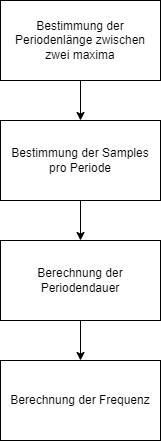
\includegraphics[scale=0.5]{Images/aufgabe9_algo2.png}
	\caption{Ablaufdiagramm des zweiten Algorithmus der Aufgabe 9}
	\label{algo2}
\end{figure}

\subsection{Aktualisierung}
Die Überlegung zu diesem Algorithmus ist vor dem Implementieren des ersten geschehen.
Hier fanden sich die selben Probleme wieder.
Ich habe in meiner Überlegung zu einfach gedacht.\par
Die Schritte zum feststellen der Anzahl der Samples können aus dem ersten Algorithmus übernommen werden.
Das wären das Einlesen der Werte, feststellen des ersten Minima und des zweiten Minima nach Anstieg.\par
Die wirkliche Änderung besteht nur in der folgenden Berechnung.
Die Samplingrate ist nun bekannt und kann verwendet werden um die Frequenz der unbekannten Sinusspannung berechnen zu können.\par
Der angepasste Algorithmus ist in Abbildung \ref{algo2.1} zu sehen.

\begin{figure}[h]
	\centering
	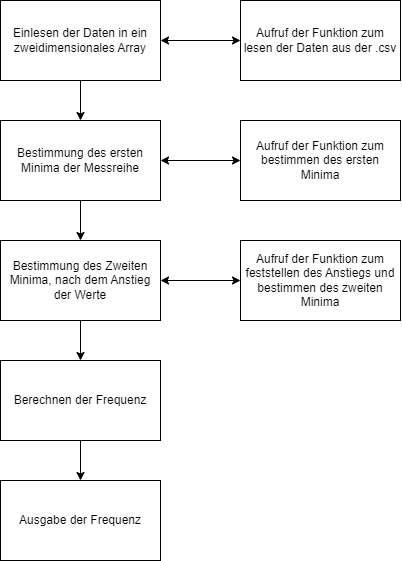
\includegraphics[scale=0.5]{Images/aufgabe9_algo2.1.png}
	\caption{Aktualisiertes Ablaufdiagramm des zweiten Algorithmus der Aufgabe 9}
	\label{algo2.1}
\end{figure}

\section{Algorithmus zur Bestimmung der Frequenz einer Rechteckspannung}
Die Frequenz der Rechteckspannung kann mit dem selben Algorithmus der zur Bestimmung der Frequenz der Sinusspannung bestimmt werden.
Beim ausprobieren hat sich allerdings ein Fehler im Algorithmus bemerkbar gemacht der bei der Sinusspannung nicht aufgetreten ist.
In den Werten der Rechteckspannung gibt es an einigen Stellen in den Minima einen Ausreißer.
Dort springt der Wert unter 14 auf 13. 
Das Problem das sich dadurch einstellt ist, das Programm nimmt diesen als erreichen des ersten Minima an.
Dieses Problem gab es bei der Sinusspannung nicht da da dort der Minimal Wert 14 war und die Ausreißer hoch auf 15 gesprungen sind.
Es muss also zusätzlich noch eine Regel Implementiert werden die bei der Rechteckspannung feststellt, dass das Minima beim ersten erreichen feststellt und die nachfolgenden Werte ignoriert.
Dazu könnte festgestellt werden an welchem Punkt die Spannung fällt und bis zu welchem Punkt.
Nach diesem Punkt müsst die Funktion dann abbrechen um das prüfen weiterer Werte zu verhindern.
Somit würde der Ausreißer nicht mit betrachtet werden.
Diese Implementierung würde definitiv auch Sinn für die Ermittlung einer Sinusspannung machen, da nicht davon ausgegangen werden kann dass bei anderen Messwert Aufnahmen dies nicht vorkommen kann.
Auch wenn dies in den bereitgestellten Messwerten nicht vorkam. 
Dies gilt auch für die Bestimmung des zweiten Minima.

\section{Repo}
In diesem Repo auf auf Gitlab befindet sich der Programmierteil der Aufgabe 9.
In diesem Repo befinden sich die Implementierungen der Algorithmen aus Aufgabe 9.
Diese dienen dazu die Samplingrate einer Aufnahme einer Oszilloskop Kurve bei bekannter Frequenz zu bestimmen und die Frequenz bei bekannter Samplingrate zu bestimmen.\par

\href{https://gitlab.thga.de/daniel.krueger/pruefung_sose_2023_aufgabe_9_algorithmen}{\textbf{LINK}}
